\documentclass[8pt]{beamer}

\newif\ifplacelogo % create a new conditional
\placelogotrue % set it to true

\usetheme{Warsaw}
\usecolortheme{rose}
\usepackage{multicol}
\usepackage{epstopdf}
\usepackage[italic]{hepnames}
\usepackage{tikz}
\usepackage{listings}
\usepackage{times}
\usepackage{amsmath}
\usepackage{verbatim}
\usepackage{hyperref}
\usepackage{bbding}
\lstset{breakatwhitespace,
language=C++,
columns=fullflexible,
keepspaces,
breaklines,
tabsize=3, 
showstringspaces=false,
extendedchars=true}

% TikZ includes!!!
\usepackage{tikz}
\usetikzlibrary{backgrounds}
\usetikzlibrary{calc}
\tikzstyle{every picture}+=[remember picture]
\input{/home/oviazlo/Desktop/beamerPresentations/myReports/latexHelpScripts/tikzGrid.tex}


\begin{document}

% custom colors
\definecolor{olive}{rgb}{0.3, 0.4, .1}
\definecolor{fore}{RGB}{249,242,215}
\definecolor{back}{RGB}{51,51,51}
\definecolor{title}{RGB}{255,0,90}
\definecolor{dgreen}{rgb}{0.,0.6,0.}
\definecolor{gold}{rgb}{1.,0.84,0.}
\definecolor{JungleGreen}{cmyk}{0.99,0,0.52,0}
\definecolor{BlueGreen}{cmyk}{0.85,0,0.33,0}
\definecolor{RawSienna}{cmyk}{0,0.72,1,0.45}
\definecolor{Magenta}{cmyk}{0,1,0,0}

\definecolor{PixelColor}{RGB}{207,232,139}
\definecolor{SCTColor}{RGB}{167,166,255}
\definecolor{TRTColor}{RGB}{250,224,140}
\definecolor{grayColor}{RGB}{153,153,153}

\newcommand{\yRefPosOne}{0.0}
\newcommand{\xRefPosOne}{0.0}
\newcommand{\yRefPosTwo}{0.0}
\newcommand{\xRefPosTwo}{0.0}
\newcommand{\yRefIncrementOne}{0.0}
\newcommand{\xRefIncrementOne}{0.0}
\newcommand{\yRefIncrementTwo}{0.0}
\newcommand{\xRefIncrementTwo}{0.0}

\graphicspath{ {/home/oviazlo/Desktop/beamerPresentations/FCCee/pictures/Sep20/} }
\DeclareGraphicsExtensions{.eps, .pdf, .png}

\newcommand{\myBox}[2][pink] {
    \noindent\colorbox{#1}{
	\textbf{#2}
    }\par
}

% For nice block (provided by Oleh)
\tikzstyle{mybox} = [draw=red, fill=blue!1, very thick,
    rectangle, rounded corners, inner sep=5pt, inner ysep=9pt]
    
\tikzstyle{PixelBox} = [draw=PixelColor, fill=blue!1, very thick,
    rectangle, rounded corners, inner sep=5pt, inner ysep=9pt]
\tikzstyle{SCTBox} = [draw=SCTColor, fill=blue!1, very thick,
    rectangle, rounded corners, inner sep=5pt, inner ysep=9pt]
\tikzstyle{TRTBox} = [draw=TRTColor, fill=blue!1, very thick,
    rectangle, rounded corners, inner sep=5pt, inner ysep=9pt]

% poster advertisement
\newcommand{\myCenterBox}[2][pink] {
   {\centering
    \noindent\colorbox{#1}{
	\textbf{#2}
    }\par
  }
}

\newcommand{\mySmallCenterBox}[2][pink] {
   {\centering
    \noindent\colorbox{#1}{
	\textbf{{\small #2}}
    }\par
  }
}

\newcommand{\myVerySmallCenterBox}[2][pink] {
   {\centering
    \noindent\colorbox{#1}{
	\textbf{{\scriptsize #2}}
    }\par
  }
}

\newcommand{\backupbegin}{
   \newcounter{finalframe}
   \setcounter{finalframe}{\value{framenumber}}
}
\newcommand{\backupend}{
   \setcounter{framenumber}{\value{finalframe}}
}

\newcommand{\myNode}{\tikz[baseline,inner sep=1pt] \node[anchor=base]}

\definecolor{light-gray}{gray}{0.95}
% poster advertisement


\title[ ECAL Photon performance \hspace{13.5em}\insertframenumber/
\inserttotalframenumber]{ ECAL Photon performance }


	\author[Oleksandr Viazlo]{Oleksandr Viazlo \\ 
% 	{\small ???}
	}
	\institute{\small CERN\\} 
	
       
	\date{20 September 2017}

% 	\logo{ \ifplacelogo \includegraphics[height=1.8cm]{./ID_week2/lund_uni-logo_s.pdf} \hspace{0.4cm} \fi}

	
   	\frame{\titlepage}

   	

\placelogofalse

%*****************************************************************************
\begin{frame}{\large \large Introduction}
 
\renewcommand{\yRefPosOne}{0.4}
\renewcommand{\xRefPosOne}{2.5}
\renewcommand{\xRefIncrementOne}{5.5}
\begin{tikzpicture}[overlay]


\node [Box] at (\xRefPosOne+2.5,\yRefPosOne) (box){%
  \begin{minipage}{\textwidth}
    \begin{itemize}
      \item Overview of the ECAL calibration procedure used for PandoraPFA package\\ \vspace{0.2cm}
      \item 10 GeV photon particle gun sample is used \\ \vspace{0.2cm}
    \end{itemize}
  \end{minipage}
};

\end{tikzpicture}

  
\end{frame}
%*****************************************************************************

%*****************************************************************************
\begin{frame}{\large \large Photon Energy Scale Bias}
\renewcommand{\yRefPosOne}{0.4}
\renewcommand{\xRefPosOne}{2.5}
\renewcommand{\xRefIncrementOne}{5.5}
\begin{tikzpicture}[overlay]

 \node[inner sep=0pt] (tmp) at (\xRefPosOne+0.5,\yRefPosOne)
  {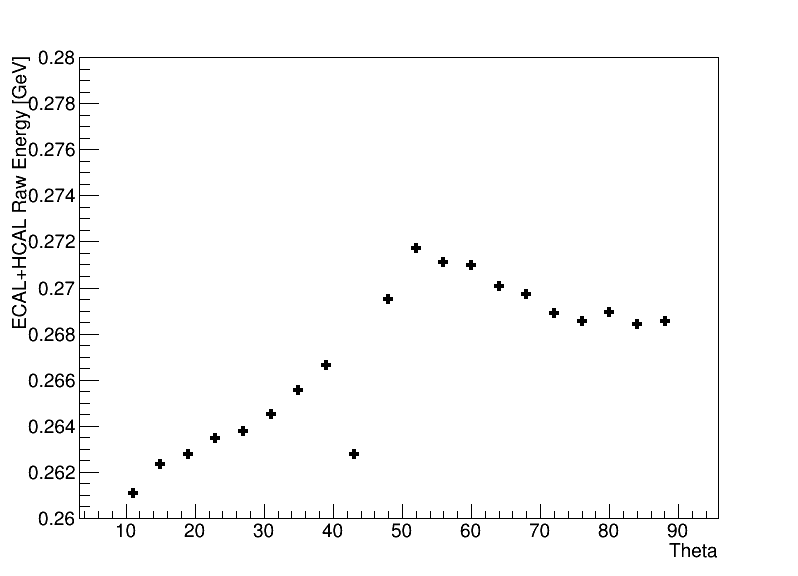
\includegraphics[width=8cm]{plot1}};

\node [Box] at (\xRefPosOne+6.5,\yRefPosOne) (box){%
  \begin{minipage}{0.55\textwidth}
    \begin{itemize}
      \item RAW Energy of all hits in ECAL+HCAL\\ \vspace{0.1cm}
    \end{itemize}
  \end{minipage}
};

\end{tikzpicture}
\end{frame}
%*****************************************************************************

%*****************************************************************************
\begin{frame}{\large \large Photon Energy Scale Bias}
\renewcommand{\yRefPosOne}{0.4}
\renewcommand{\xRefPosOne}{2.5}
\renewcommand{\xRefIncrementOne}{5.5}
\begin{tikzpicture}[overlay]

 \node[inner sep=0pt] (tmp) at (\xRefPosOne+0.5,\yRefPosOne)
  {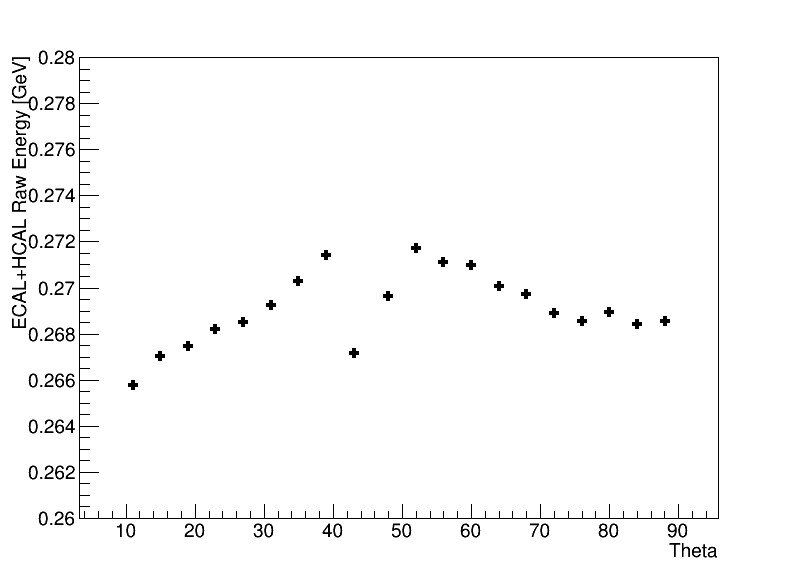
\includegraphics[width=8cm]{plot2}};

\node [Box] at (\xRefPosOne+6.5,\yRefPosOne) (box){%
  \begin{minipage}{0.55\textwidth}
    \begin{itemize}
      \item RAW Energy of all hits in ECAL+HCAL\\ \vspace{0.1cm}
      \item Endcap energy correction factor (1.018)\\ \vspace{0.1cm}
    \end{itemize}
  \end{minipage}
};

% \node [Box] at (\xRefPosOne+0.5,\yRefPosOne+2) (box){%
% \myCenterBox{Effect in Endcap: 2$\%$, in Barrel: 1.2$\%$}
% }; 

\end{tikzpicture}
\end{frame}
%*****************************************************************************

%*****************************************************************************
\begin{frame}{\large \large Photon Energy Scale Bias}
\renewcommand{\yRefPosOne}{0.4}
\renewcommand{\xRefPosOne}{2.5}
\renewcommand{\xRefIncrementOne}{5.5}
\begin{tikzpicture}[overlay]

 \node[inner sep=0pt] (tmp) at (\xRefPosOne+0.5,\yRefPosOne)
  {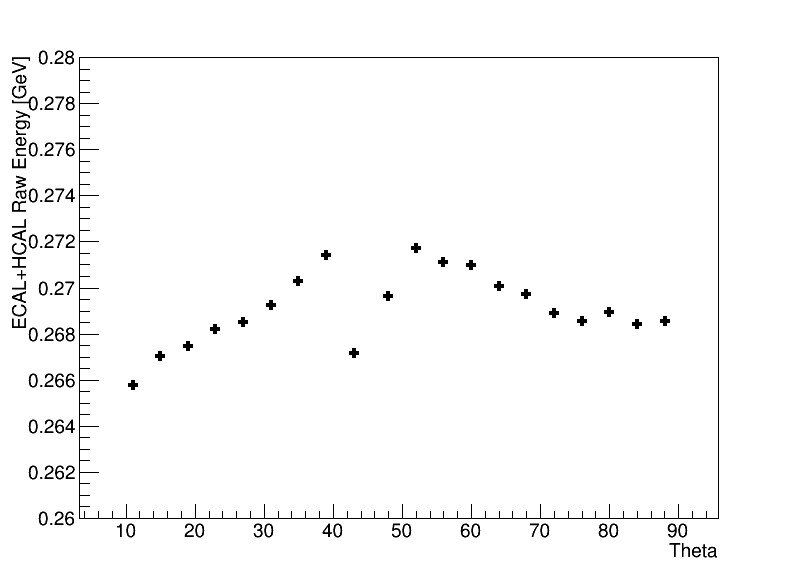
\includegraphics[width=8cm]{plot2}};

\node [Box] at (\xRefPosOne+6.5,\yRefPosOne) (box){%
  \begin{minipage}{0.55\textwidth}
    \begin{itemize}
      \item RAW Energy of all hits in ECAL+HCAL\\ \vspace{0.1cm}
      \item Endcap energy correction factor (1.018)\\ \vspace{0.1cm}
    \end{itemize}
  \end{minipage}
};

\node [Box] at (\xRefPosOne+0.5,\yRefPosOne+2) (box){%
\myCenterBox{Effect in Endcap: 2$\%$, in Barrel: 1.2$\%$}
}; 

\end{tikzpicture}
\end{frame}
%*****************************************************************************

%*****************************************************************************
\begin{frame}{\large \large Photon Energy Scale Bias}
\renewcommand{\yRefPosOne}{0.4}
\renewcommand{\xRefPosOne}{2.5}
\renewcommand{\xRefIncrementOne}{5.5}
\begin{tikzpicture}[overlay]

 \node[inner sep=0pt] (tmp) at (\xRefPosOne+0.5,\yRefPosOne)
  {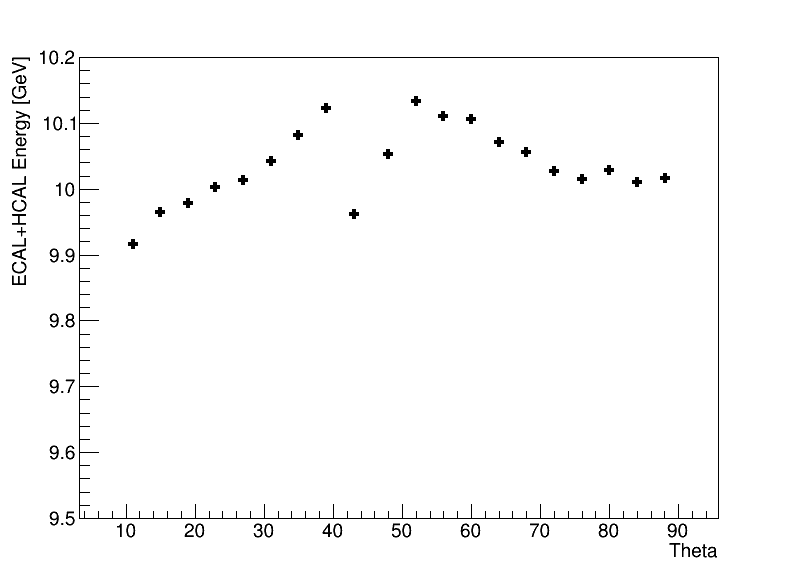
\includegraphics[width=8cm]{plot3}};

\node [Box] at (\xRefPosOne+6.5,\yRefPosOne) (box){%
  \begin{minipage}{0.55\textwidth}
    \begin{itemize}
      \item RAW Energy of all hits in ECAL+HCAL \\ \vspace{0.1cm}
      \item Endcap energy correction factor (1.018) \\ \vspace{0.1cm}
      \item Calibration coefficient for ECAL (37.44) \\ \vspace{0.1cm}
    \end{itemize}
  \end{minipage}
};

\end{tikzpicture}
\end{frame}
%*****************************************************************************

%*****************************************************************************
\begin{frame}{\large \large Photon Energy Scale Bias}
\renewcommand{\yRefPosOne}{0.4}
\renewcommand{\xRefPosOne}{2.5}
\renewcommand{\xRefIncrementOne}{5.5}
\begin{tikzpicture}[overlay]

 \node[inner sep=0pt] (tmp) at (\xRefPosOne+0.5,\yRefPosOne)
  {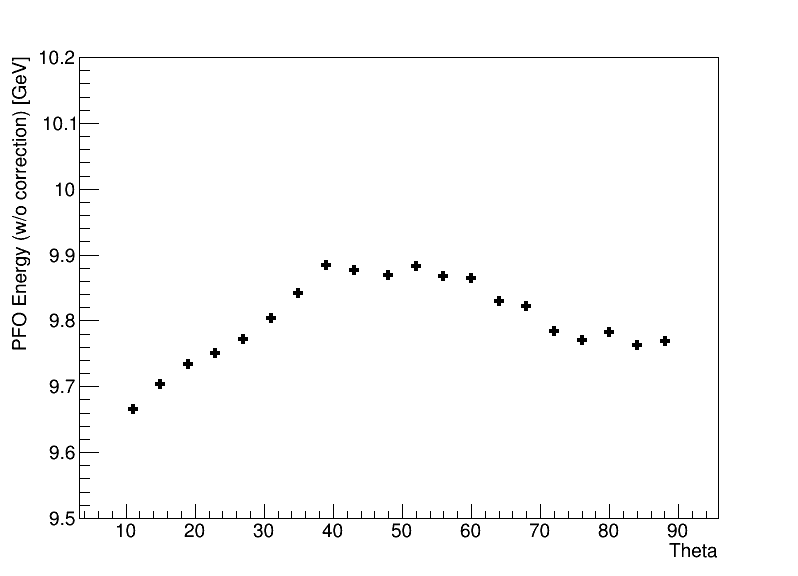
\includegraphics[width=8cm]{plot4}};

\node [Box] at (\xRefPosOne+6.5,\yRefPosOne) (box){%
  \begin{minipage}{0.55\textwidth}
    \begin{itemize}
      \item RAW Energy of all hits in ECAL+HCAL \\ \vspace{0.1cm}
      \item Endcap energy correction factor (1.018) \\ \vspace{0.1cm}
      \item Calibration coefficient for ECAL (37.44) \\ \vspace{0.1cm}
      \item PFO clusterization algorithm \\ \vspace{0.1cm}
    \end{itemize}
  \end{minipage}
};

\end{tikzpicture}
\end{frame}
%*****************************************************************************

%*****************************************************************************
\begin{frame}{\large \large Photon Energy Scale Bias}
\renewcommand{\yRefPosOne}{0.4}
\renewcommand{\xRefPosOne}{2.5}
\renewcommand{\xRefIncrementOne}{5.5}
\begin{tikzpicture}[overlay]

 \node[inner sep=0pt] (tmp) at (\xRefPosOne+0.5,\yRefPosOne)
  {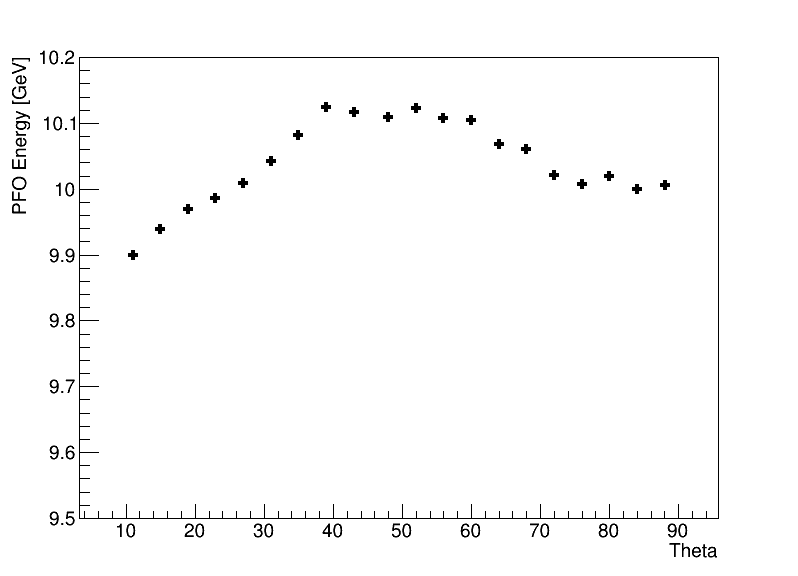
\includegraphics[width=8cm]{plot5}};

\node [Box] at (\xRefPosOne+6.5,\yRefPosOne) (box){%
  \begin{minipage}{0.55\textwidth}
    \begin{itemize}
      \item RAW Energy of all hits in ECAL+HCAL \\ \vspace{0.1cm}
      \item Endcap energy correction factor (1.018) \\ \vspace{0.1cm}
      \item Calibration coefficient for ECAL (37.44) \\ \vspace{0.1cm}
      \item PFO clusterization algorithm \\ \vspace{0.1cm}
      \item PFO photon energy correction (1.024) \\ \vspace{0.1cm}
    \end{itemize}
  \end{minipage}
};

\end{tikzpicture}
\end{frame}
%*****************************************************************************

%*****************************************************************************
\begin{frame}{\large \large Photon Energy Scale Bias}
\renewcommand{\yRefPosOne}{0.4}
\renewcommand{\xRefPosOne}{2.5}
\renewcommand{\xRefIncrementOne}{5.5}
\begin{tikzpicture}[overlay]

 \node[inner sep=0pt] (tmp) at (\xRefPosOne+0.5,\yRefPosOne)
  {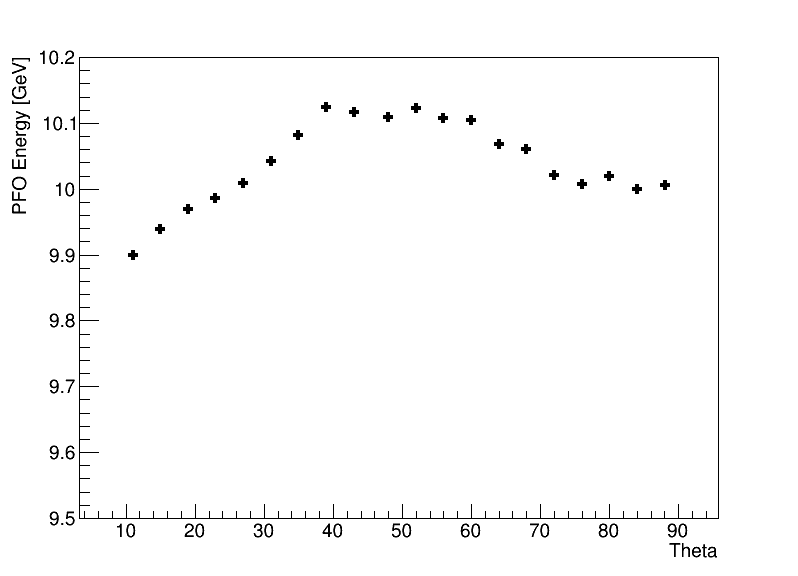
\includegraphics[width=8cm]{plot5}};

\node [Box] at (\xRefPosOne+6.5,\yRefPosOne) (box){%
  \begin{minipage}{0.55\textwidth}
    \begin{itemize}
      \item RAW Energy of all hits in ECAL+HCAL \\ \vspace{0.1cm}
      \item Endcap energy correction factor (1.018) \\ \vspace{0.1cm}
      \item Calibration coefficient for ECAL (37.44) \\ \vspace{0.1cm}
      \item PFO clusterization algorithm \\ \vspace{0.1cm}
      \item PFO photon energy correction (1.024) \\ \vspace{0.1cm}
    \end{itemize}
  \end{minipage}
};

\node [Box] at (\xRefPosOne+0.5,\yRefPosOne-1) (box){%
\myCenterBox{Effect in Endcap: 2$\%$, in Barrel: 1.2$\%$}
}; 

\node [Box] at (\xRefPosOne+0.5,\yRefPosOne-1.5) (box){%
\myCenterBox{Effect propagates from RAW energy distribution}
}; 

\end{tikzpicture}
\end{frame}
%*****************************************************************************

%*****************************************************************************
\begin{frame}{\large \large Photon Energy Scale Bias: CLIC}
 
\renewcommand{\yRefPosOne}{0.4}
\renewcommand{\xRefPosOne}{2.5}
\renewcommand{\xRefIncrementOne}{5.5}
\begin{tikzpicture}[overlay]

 \node[inner sep=0pt] (tmp) at (\xRefPosOne,\yRefPosOne)
  {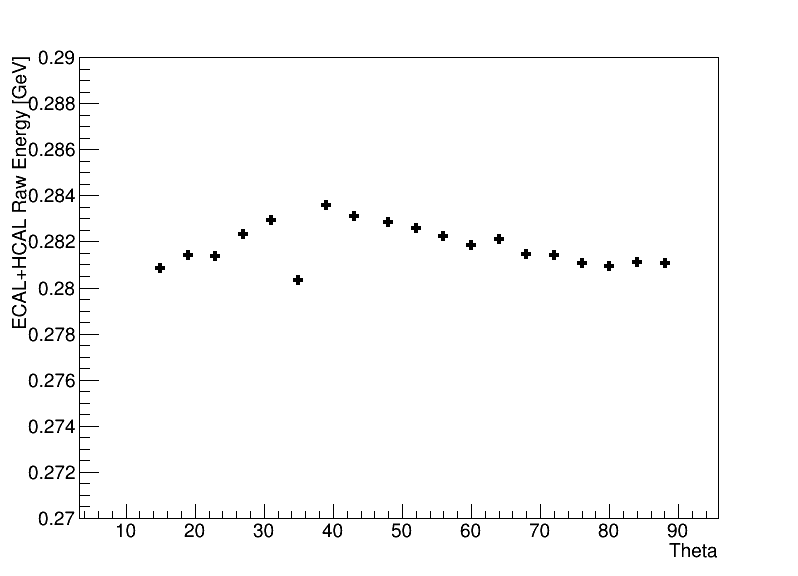
\includegraphics[width=6.5cm]{CLIC_plot1.png}};

 \node[inner sep=0pt] (tmp) at (\xRefPosOne+6,\yRefPosOne)
  {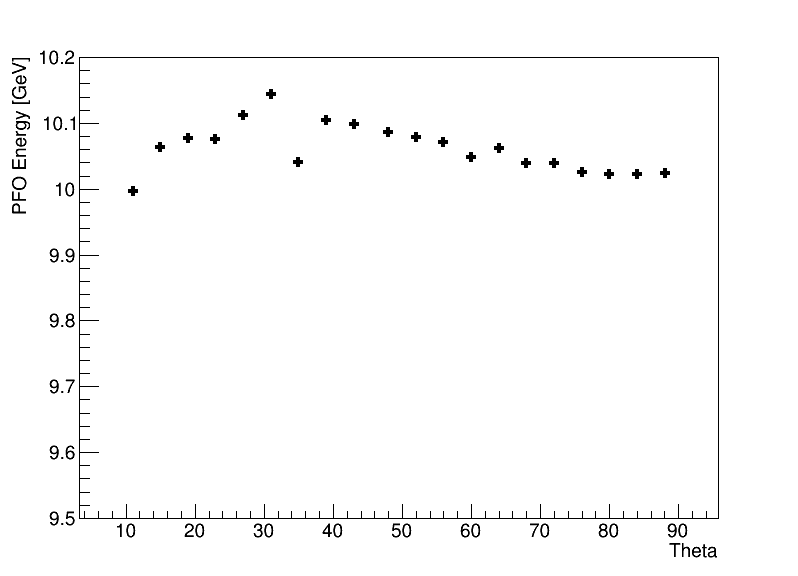
\includegraphics[width=6.5cm]{CLIC_plot2.png}};

% 
\node [Box] at (\xRefPosOne,\yRefPosOne+1.5) (box){%
\myCenterBox{CLIC}
};

\node [Box] at (\xRefPosOne+2.5,\yRefPosOne-3.8) (box){%
  \begin{minipage}{\textwidth}
    \begin{itemize}
      \item Same calibraiton procedure is used for CLIC detector
      \item Effect both in Endcap and Barrel is $\sim$1$\%$ level
    \end{itemize}
  \end{minipage}
};

\end{tikzpicture}

  
\end{frame}
%*****************************************************************************

%*****************************************************************************
\begin{frame}{\large \large Summary}
 
\renewcommand{\yRefPosOne}{0.4}
\renewcommand{\xRefPosOne}{2.5}
\renewcommand{\xRefIncrementOne}{5.5}
\begin{tikzpicture}[overlay]

 \node[inner sep=0pt] (tmp) at (\xRefPosOne,\yRefPosOne)
  {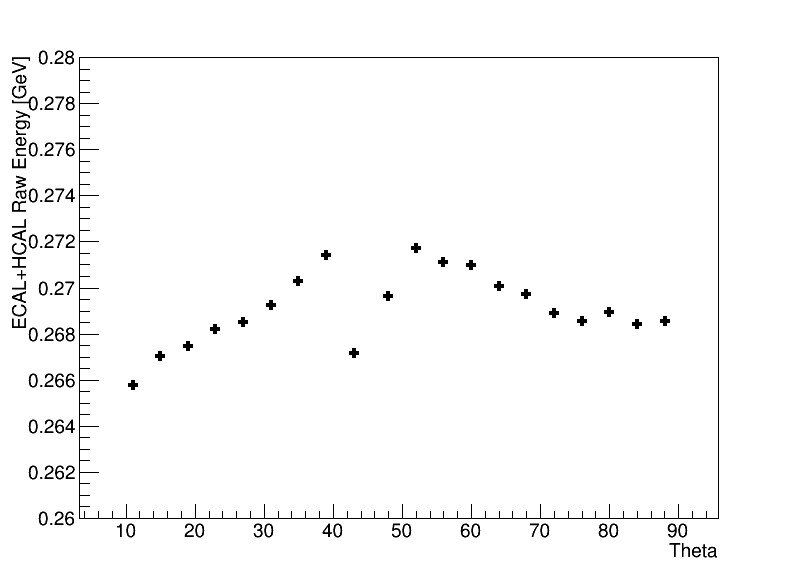
\includegraphics[width=6.5cm]{plot2.png}};

 \node[inner sep=0pt] (tmp) at (\xRefPosOne+6,\yRefPosOne)
  {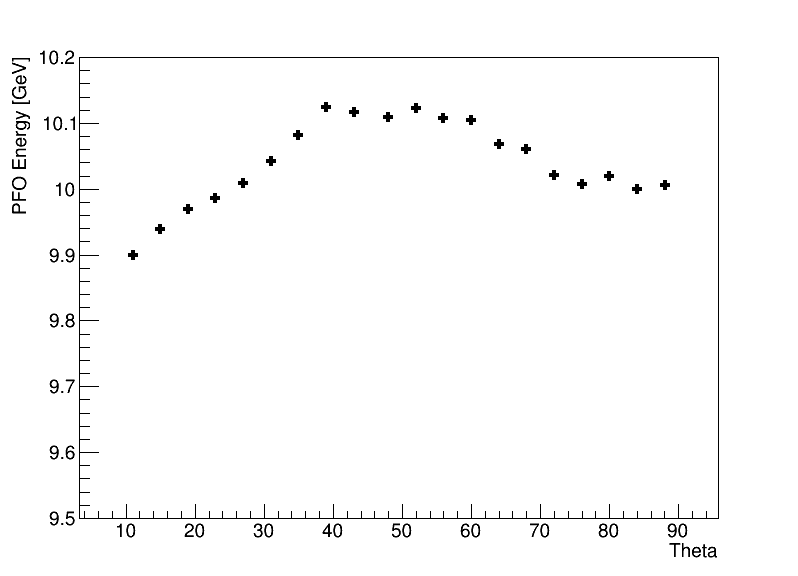
\includegraphics[width=6.5cm]{plot5.png}};

% 
\node [Box] at (\xRefPosOne,\yRefPosOne+1.5) (box){%
\myCenterBox{FCCee}
};

\node [Box] at (\xRefPosOne+2.5,\yRefPosOne-3.8) (box){%
  \begin{minipage}{\textwidth}
    \begin{itemize}
      \item Such callibration procedure is used both by ILD and CLIC collaborations
      \item Current implementation of the PandoraFFA package doesn't support theta and 
      energy dependence of the calibraiton constants
      \item The same procedure is used for HCAL (with a few additional steps)
    \end{itemize}
  \end{minipage}
};

\end{tikzpicture}

  
\end{frame}
%*****************************************************************************

\end{document}

